% TODO Aaron thinks we should say: There are two well known devices used in
% skimmers. IN this section we will see if those devices are easily
% distinguishable in the Bluetooth environment around gas stations.

% *Data collection methodology* This data comes from two sources (1) a
% crowdsourced collection of data across multiple metropolitan areas around the
% US., and becuase we know in certain states which are the most vulernable
% pumps, we did on did a focused data collection that in one metropolitan area.
% (Street view mention) *Summary plot:* How many gas stations seen in each
% state

% Q1: Are classic unclassified common at gas stations?
% A1: Unclassified are much less common than classic in general, becuase most classic car stereos or phones (numbers based on major class). Most gas stations have 0 classic devices.

% Q2: Of all unclassified classics, how many match the manfacturers of known skimmers.
% A2: Most unclass classic are one MFG, which happens to be used in skimmers, there are others as well, many appear as not having a known mfg.

% Q3: Of roving networks, what is the breakdown of types of devices by name?
% Q3: Name clustering results show that most are ODBII or Smog, and a few are other or default.
%  - FWD pointer - obviously this means they could hide the name in the noise. We will dsicuss in the next section what we can do about that and how much they can really hide by doing it.

% Summary, it does seem feasible to detect skimmers by matching characteristics
% of known Bluetooth modules, but the modules used in skimmers are popular,
% detection will need to exclude a rather large number of devices that appear
% in a similar way as skimmers do, and also are located at gas stations, but
% are not skimmers.


%!TEX root = paper.tex
\section{Results}
\label{sec:results}

In the previous sections, we have established that there are certain commodity Bluetooth modules used in skimmers. We then design Bluetana to record Bluetooth scan information to detect these skimmers. Bluetana enabled us to perform a large-scale survey of gas stations in the past year, and successfully detect 22 skimmers across multiple cities in US. In this section, we present the results of our survey as a series of questions aimed at understanding whether Bluetooth scan information can be used to effectively detect these modules.

\subsection{The data collection} %{{{

We recruited known individuals in metropolitan areas across 5 different states in the US. Using our app, the recruits were able to perform a large scale data collection of the Bluetooth environment around gas stations. The data collectors included researchers, rideshare drivers and AZDWM inspectors, who visited several gas stations over a period of time.

Southern California, and San Diego county in particular, is known to be a hotbed of skimmer activity. To do a wider study of multiple gas stations in the county, we inspected all gas stations which have a particular vulnerable style of gas pump - three upper doors with card reader access through universal key. By obtaining coordinates of all gas stations from GIS databases, and inspecting Google Street View images, we were able to identify 208 in particular that fit this criteria (Figure \ref{fig:google_streetview}) 

\begin{figure}
\centering
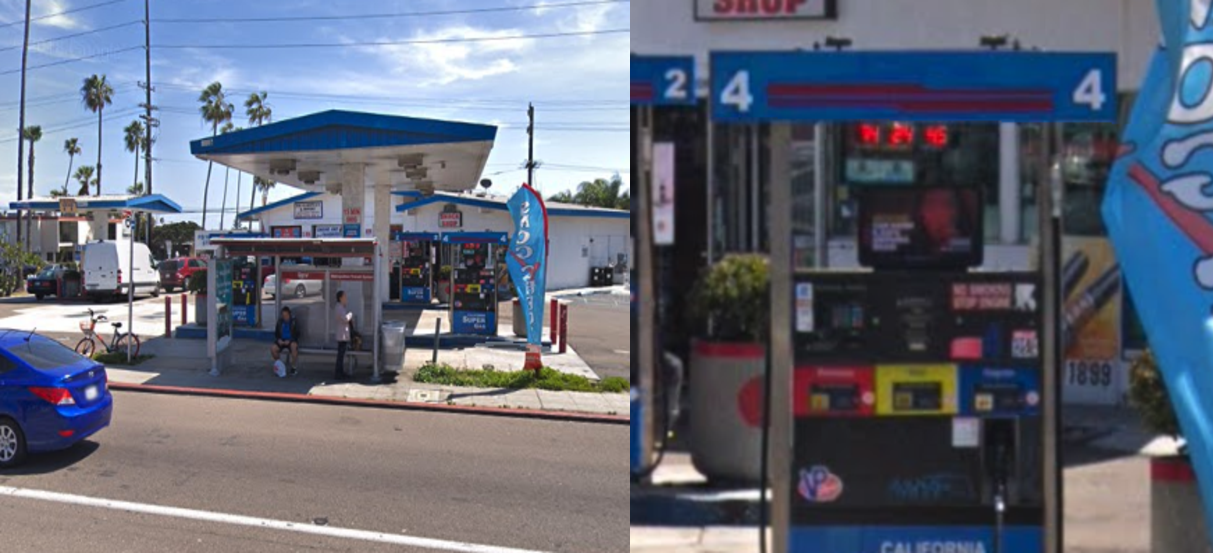
\includegraphics[width=\linewidth]{fig/googlestreetview.pdf}
\caption{
  \label{fig:google_streetview}
  Image on left is a Google Street view from the street. Image on right is zoomed into the dispenser, clearly showing the 3-door style pump
}
\end{figure}

We analyze the data collected to answer questions that helps us get a better understanding of the heuristics that can be used to detect skimmers. To start off, we try and see if it is realistic to use Bluetooth scan information for detecting skimmers.

\subsection {Are Bluetooth devices so common at gas stations, that hiding a skimmer is easy?}

Table \ref{tab:total_gs_bl} is a summary of the Bluetooth data collected by visiting gas stations across 5 states in the US. We only consider gas stations in which the observer was within a 200 ft radius of the gas station for 30s or more, and show data collected in the first 30s.
    
\begin{table}
\centering
\resizebox{1\columnwidth}{!}{
\begin{tabular}{r|c|c|c|c|c}
%\cline{2-8}
%\multicolumn{1}{c|}{} & \multicolumn{8}{c|}{\cellcolor{black}\textcolor{white}{\textbf{\# of Gas Stations}} \\
% A & \textbf{None} & \textbf{ModuleA\n only} & \textbf{ModuleB\n only} & \textbf{Both} & T \\
\multicolumn{1}{c|}{} & \textbf{CA} & \textbf{AZ} & \textbf{MD} & \textbf{NC} & \textbf{IL}\\
\hline
\multicolumn{1}{r|}{Observation period (months)}    &  12 &  1 &  6 & 5 & 2 \\
\multicolumn{1}{r|}{\# of fuel stations surveyed}    &  613 &  92 &  46 & 28 & 28 \\
\multicolumn{1}{r|}{\# of Bluetooth devices seen}   &  536  & 110  & 46 & 35 & 23  \\
\hline
\end{tabular}
}

\caption{Distribution of gas stations and Bluetooth devices seen by state. The possibility of seeing a classic Bluetooth device at a gas station is fairly low.}
\label{tab:total_gs_bl}
\end{table}

The table shows that presence of multiple Bluetooth devices at any given gas station is rare, and thus hiding a particular Bluetooth skimmer is not easy. A small number of Bluetooth devices also makes it very feasible at any gas station to use Bluetooth scanning information for skimmer detection

Starting with information that modules RN and HC are commonly used in skimmers, we analyze our dataset to identify Bluetooth characteristics that can help detect these modules in the wild.

\subsection {What are the set of Bluetooth characteristics that can identify these modules?}

Bluetooth device discovery can provide information that can be used to look for skimmers. From our dataset analysis, we identify the following properties

\subsubsection {MAC address}

For RN modules, we observe the OUI to be consistently \texttt{00:06:66} and therefore a reliable heuristic. However, HC modules from different manufacturers, despite having the same Bluetooth chipset and PCB design exhibit different MAC prefixes, which appear to be globally unique (lowest bits of most significant byte are unset)\cite{OUIguidelines}, but are unassigned to any entity. Taking these insights into consideration, Table \ref{tab:Modules_state} provides a summary of how many RN and HC modules we observe at gas stations by state.

\begin{table}
\centering
\scriptsize
\resizebox{1\columnwidth}{!}{
\begin{tabular}{c|c}
\textbf{Source} & \textbf{MAC address range} \\
\hline
A & 20:18:08:XX:XX:XX \\
B & 98:D3:32:XX:XX:XX \\
C & 20:13:07:XX:XX:XX \\
\hline
\end{tabular}
}
\caption{Different MAC ranges observed for HC modules purchased from different sources}
\label{tab:ModuleB_MAC}
\end{table}

\begin{table}[]
\centering
\scriptsize
\resizebox{1\columnwidth}{!}{
\begin{tabular}{r|c|c|c|c|c}
\multicolumn{1}{c|}{} & \textbf{CA} & \textbf{AZ} & \textbf{MD} & \textbf{NC} & \textbf{IL} \\
\hline
\multicolumn{1}{r|}{\# of RN}    &  40  &  18  &  4 & 2 & 2\\
\multicolumn{1}{r|}{\# of HC}   &  2  &  4  & 2 & 0 & 0  \\
\hline
\end{tabular}
}
\caption{Distribution of Bluetooth modules observed per state}
\label{tab:MAC_state}
\end{table}

\subsubsection{Class of Device}

As discussed in previous section, the Class of Device (CoD) across all RN and HC regardless of manufacturer) modules is known to be \texttt{Uncategorized} out of the box. While CoD can be modified in these modules, our data shows that we rarely observed any RN or HC device that is not \texttt{Uncategorized}, and the the ones we did were not in the vicinity of gas stations. Therefore this appears to be a property which criminals are not exploiting to hide their skimmers, and therefore something we can exploit to find them. Table \ref{tab:Modules_state} shows the number of uncategorized HC and RN devices we observed in the vicinity of gas stations.


\begin{table}[]
\centering
\scriptsize
\resizebox{1\columnwidth}{!}{
\begin{tabular}{r|c|c|c|c|c}
\multicolumn{1}{c}{} & \textbf{CA} & \textbf{AZ} & \textbf{MD} & \textbf{NC} & \textbf{IL} \\
\hline
\multicolumn{1}{r|}{\# of uncategorized}    &  38  &  16  &  3 & 0 & 0\\
\hline
\end{tabular}
}
\caption{Distribution of Uncategorized RN and HC modules observed per state}
\label{tab:Modules_state}
\end{table}

\subsubsection{Device Name}
While collecting data, we encountered skimmers attempting to disguise themselves by using innocuous names (\textit{111}) or something an average user might want to avoid (\textit{Police Survey 11}). 

However, Lavelle et al[\cite{bluetoothnames}] claimed through controlled studies in their work that over 43\% of device users adopt either default product names or use a name that indicates the function of the device. This implies that device names may provide some clues about other legitimate products that also appear as skimmers. We discussion more about this in a later subsection

\paragraph{Summary}
In this section we have identified the Bluetooth parameters that can be used to identify a particular Bluetooth modules. However, we know that these parameters can be changed with varying levels of difficulty, with device name being the easiest to modify. As discussed previously, majority of these criminals operate with a low level of technical skill, and therefore making the effort to change parameters like MAC address and CoD for their exfil medium doesnt seem likely. 

Given this, we make a hypothesis at this stage : Criminals use RN and HC modules with factory default MAC address and CoD in skimmers. In the following subsections we attempt to provide evidence to support the hypothesis with our data. While at this stage default names appear to be unreliable for skimmer identification because of ease of modification, we shall discover eventually that they work well a lot of cases.


\subsection {So how prevalent are gas stations with any of the modules within their premises?}

In the previous subsection, we have defined the MAC address and CoD as relevant parameters in our search for skimmers. We use these parameters in table \ref{tab:gs_hitlistmatch} to identify number of gas stations where we any RN or HC module. In the table we also provide a lookahead as to how many eventually end up being skimmers.

\begin{table}
\centering
\resizebox{1\columnwidth}{!}{
\begin{tabular}{cr|c|c|c|l}
 \multicolumn{2}{c}{} & \textbf{Mod$_A$} & \textbf{Mod$_B$} & \textbf{Mod$_{A\&B}$} & \textbf{Neither} \\
\hline
\multicolumn{2}{r}{California}    &  \cellcolor{lightgray}23/4  &  \cellcolor{lightgray}2/1  &  0/0 &  588 \\
\multicolumn{2}{r}{Arizona}   &  10/0  &  \cellcolor{lightgray}1/1  &  \cellcolor{lightgray}1/1 &  80  \\
\multicolumn{2}{r}{Maryland}   &  2/0  &  \cellcolor{lightgray}1/1  &  0/0   &  43 \\
\multicolumn{2}{r}{Illinois}   &  0/0  &  0/0  &  0/0  &  28 \\
\multicolumn{2}{r}{N. Carolina}  & 0/0 & 0/0 & 0/0 & 28 \\
\hline
\multicolumn{1}{c}{\cellcolor{lightgray}} & \multicolumn{5}{l}{= skimmers recovered at one or more gas stations} \\ 
\end{tabular}
}

\caption{Distribution of number of gas stations in each state where we observed one or more Module $x$ (Mod$_x$) shown as A/B (A: Number of gas stations where a module was seen, B: Number of gas stations where skimmers were eventually recovered)}
\label{tab:gs_hitlistmatch}
\end{table}

As can be seen from the table that the number of gas stations with skimmers is a small number, reiterating the fact that these modules are truly a needle in a haystack. The key insight here is that if we do see any such module at a gas station, it warrants an investigation but not necessarily implies that there exists a skimmer. So the question is short of opening up all the gas pumps, do we have any other information that we can use to identify what these suspect modules are?

\subsection {How do you eliminate something that looks like a skimmer but is not?}

Using our default parameters for HC and RN, we have identified 62 different suspect modules across the gas stations shown in Table \ref{tab:gs_hitlistmatch}. We could have chosen to call in all of these modules, but as the table also shows we would have been wrong in a majority of the cases. In this subsection we talk about additional Bluetooth scan info - Device Name and RSSI, and how these can be used to reduce our suspect list.

\subsubsection{Device Name}
As discussed previously, there are some detection methods that use default device names as a method for identifying skimmers in the wild. However knowledge of these modules suggests that device names are easily modifiable and therefore not reliable for clues on skimmer detection. It is required that we test this theory out.

As we have discussed previously, device names of legitimate products may actually help in removing those from the suspect list. We study this aspect of device identification on our list of suspect devices, by grouping names using name prefix clustering.

\begin{figure}
\centering
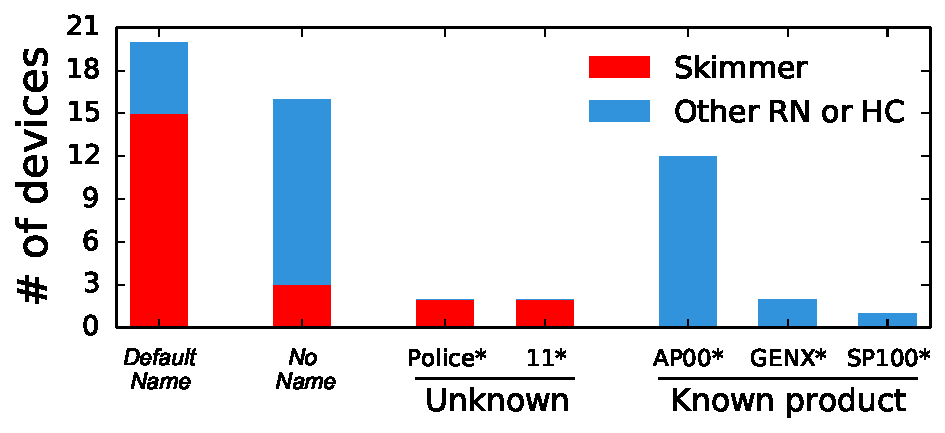
\includegraphics[width=\linewidth]{plots/bar_plot_name_cluster.pdf}
\caption{
  \label{fig:barplot_name_cluster}
  These modules appear to be used in skimmers as well as other legitimate products commonly seen at gas stations. 
}
\end{figure}

Figure \ref{fig:barplot_name_cluster} groups the different device names associated with HC and RN modules that use the MAC and CoD parameters defined in the previous section. We also mark how many of them actually ended up being skimmers. There are certain insights that this name clustering reveals :

\begin{prettylist}
	%
	\item \textbf{Legitimate products use these modules.} For instance, AP100* is a known name associated with On-Board Diagnostic readers that are found at smog check centres. SP100* and GENX* are the common product names of Bluetooth converter systems for car stereos. 
	%
	\item \textbf{A large number of recovered skimmers use default name.} 75\% of modules with default RN or HC module name ended up being recovered as skimmers and therefore this in itself can be a reasonable marker for a skimmer. Note, however there are other kinds of module names that also can be skimmers, so we must be careful.
	%
	\item \textbf{Wierd names had sequential patterns.} We saw two "pairs" of module names at two different gas stations - \textit{(Police Survey 11, Police Survey 15)} and \textit{(110,111)}. While the names are random, they seem to be part of a sequence. Information from USSS tells us that these criminals are known to plant a number of these skimmers across multiple gas stations in a single \textit{skimming} run, and therefore the idea of sequential identifiers existing is possible. In fact in both the mentioned cases, all modules did turn out to be skimmers.
\end{prettylist}

Device Names do seem to have strong implications about the intended application of the Bluetooth device. However, we are still faced with the question of confidence of names : How do we confirm that something that shows up as an AP00* device is not simply a masked skimmer? To answer this question we look into one final aspect of Bluetooth scan information - RSSI

\subsubsection{RSSI}
As described in previous sections, Bluetana enables fine grained localization of Bluetooth modules by real time RSSI updates. We used this feature during data collection wherein we asked our observers to localize all observed RN and HC devices to gas dispensers. Figure \ref{fig:rssi_motivation} shows Google Maps images of our localization attempt. Image on the left shows a skimmer module with default name close to the gas pumps, whereas image on the right is an AP00* device located in and around the smog check clinic.

\begin{figure}
\centering
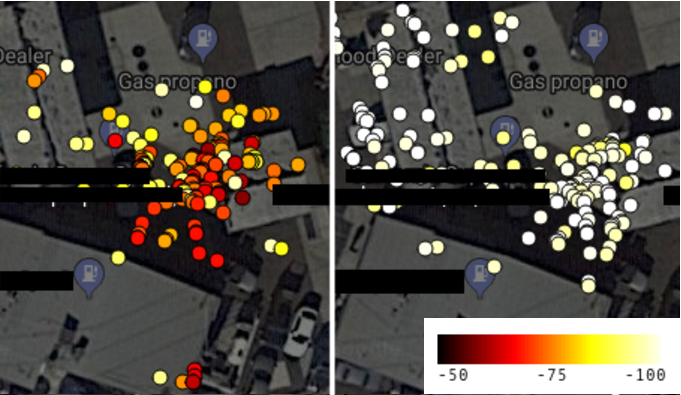
\includegraphics[width=\linewidth]{fig/rssi_motivation.pdf}\\
\caption{
\label{fig:rssi_motivation}
Image on left has Bluetana records for a skimmer located near gas dispensers, whereas on the right is an AP00* device that is localized to the smog check clinic, as expected
}
\end{figure}

RSSI localization provides a final confirmation to clearly earmark suspect devices which are very likely skimmers. Additionally we were able to confirm our hypothesis about product names. Clearly we see that all the device names of legitimate products we have observed are indeed not located close to the gas dispensers, and therefore device names while modifiable are still a relevant heuristic for culling down the suspect list.

An interesting reverse implication also can be obtained from the combination of RSSI and device names. If criminals were to hide their skimmers using names of products like AP00*, and RSSI localization puts them near actual gas dispensers, then that is definitely questionable.


\subsection {So how accurate is our hypothesis of searching for default MAC address and CoD?}

So far we have looked at the various Bluetooth characteristics that can be used to identify skimmers. Using them we have clearly identified 28 different modules we suspect to be skimmers. But most of our search was based off an initial hypothesis that criminals are predominately using RN and HC modules with a defined MAC address and CoD patterns. In this subsection we provide validation of our methodology by using ground truth data obtained from relevant authorities. We work with separate agencies outside and in Arizona and we present ground truth accordingly.

\subsubsection{Outside Arizona}
We have a collaboration with the US Secret Service, who were willing to investigate any skimmers that we report across the US. Because we didnt want to impose additional investigations on law enforcement, we did an additional check at all the locations by driving back to the gas station on the same day to confirm whether the device we saw earlier in the day still existed. 

We saw out of 20 modules, 3 devices did not show up again in Bluetana scans. For all the other devices we reported, SS authorities went in and inspected all gas pumps in every single gas station. They were able to recover the exact number of skimmers as we reported even after inspecting all the pumps. Our success rate at this point can be evaluated to 85\% with the 3 devices counting towards our false positives.

\textbf{So why were there false positives?} As we have already seen during our evaluation that a variety of applications are designed using RN and HC modules. Products such as car stereos and Bluetooth headsets are typically associated with transient traffic at gas stations. Because vehicles are parked close enough to the gas dispenser in certain cases, we didnt have the opportunity to go close enough to the dispenser to localize accurately enough, thus causing false positives.  

Despite a dynamically changing gas station Bluetooth environment, we were able to achieve an \textbf{accuracy of 85\%} in detecting skimmers

\subsubsection{What about our false negatives though?: Arizona}

To figure out how successful Bluetana was in a real world investigative scenario. we partnered with the state inspectors in Arizona Weights and Measures. As mentioned before state inspectors do regular complete inspections of gas stations based on routine or complaints. We deployed our app to 3 inspectors, who used it during regular inspections as well as to discover skimmers for impromptu inspections.

\begin{table}
\centering
\scriptsize
\resizebox{1\columnwidth}{!}{
\begin{tabular}{r|c}
%\cline{2-8}
%\multicolumn{1}{c|}{} & \multicolumn{8}{c|}{\cellcolor{black}\textcolor{white}{\textbf{\# of Gas Stations}} \\
% A & \textbf{None} & \textbf{ModuleA\n only} & \textbf{ModuleB\n only} & \textbf{Both} & T \\
\multicolumn{1}{c|}{} & \textbf{\#} \\
\hline
\multicolumn{1}{r|}{\# of reports}    &  27 \\
\multicolumn{1}{r|}{True positive}   &  5  \\

\multicolumn{1}{r|}{True negative} & 32  \\
\multicolumn{1}{r|}{False positive}   &  2   \\
\multicolumn{1}{r|}{False negative} & 2 \\
\hline
\end{tabular}
}
\caption{Our accuracy rates in Arizona across inspections done in one month}
\label{tab:arizona_falsepositive}
\end{table}

Table shows the accuracy rate of Bluetana being used across the month of November by AZDWM. For a conservative estimate, we have even included all inspections when Bluetana was used on or any day prior to the day of inspection at the same location. We achieved a high accuracy in not only detecting the presence of skimmers, but also in detecting true negatives. 

\textbf{What about the false negatives?} There were two instances where we observed false negatives. In the first case, Bluetana was used at a location 11 days prior to the actual inspection. The actual inspection was performed by a different inspector who did not use Bluetana on the day of the inspection. As there is no data to suggest when the skimmer was planted, it is difficult to figure out whether it is truly a false negative. However, we still decide to report it.

In the other false negative case, the inspector did not visit but drove past a particular gas station , with the Bluetana app running on his phone. This happened 2 days before the skimmer was recovered. Even if we assume the skimmer was already in place, the total time the inspector was in the vicinity of the gas station was less than 10s, which is not sufficient to run a single complete discovery cycle for Android, and therefore this can have possibly contributed to missing the skimmer.

\subsection {If the inspectors had not used Bluetooth, would they have missed something?}


\begin{figure}
\centering
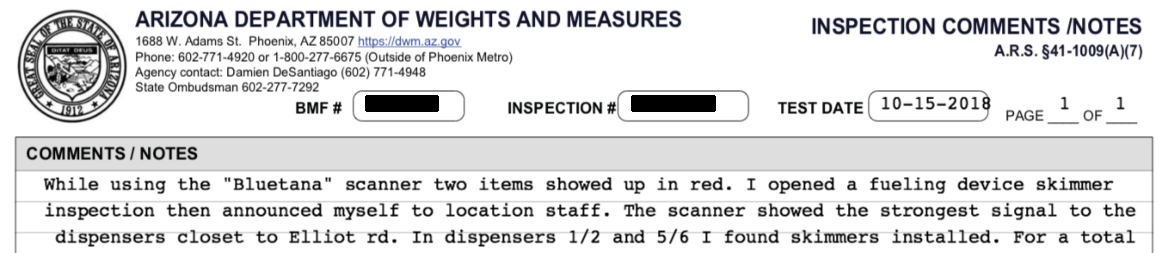
\includegraphics[width=1\linewidth]{fig/arizona_report.pdf}
\caption{ine
\label{fig:hitlist_devices}
Arizona inspection report when Bluetana scanning was instrumental in identifying a gas station not scheduled for inspection
}
\end{figure}

\begin{table}[]
\centering

\resizebox{1\columnwidth}{!}{
\begin{tabular}{r|c|c|c}
\multicolumn{1}{c|}{} & \textbf{Bluetana} & \textbf{SkimPlus} & \textbf{SkimmerScanner} \\
\hline
\multicolumn{1}{r|}{MAC address}    & Yes  &  Yes  & No \\
\multicolumn{1}{r|}{CoD}   &  Yes  &  No  & No  \\
\multicolumn{1}{r|}{Device Names} & Yes & No & Yes$^1$ \\
\multicolumn{1}{r|}{RSSI} & Yes & Yes$^2$ & No \\
\multicolumn{1}{r|}{Realtime RSSI updates} & Yes & No & No \\
\hline
\multicolumn{1}{r}{1 :} & \multicolumn{3}{l}{Only searches for string "HC-05"} \\
\multicolumn{1}{r}{2 :} & \multicolumn{3}{l}{Limited and coarse grained} \\
\end{tabular}
}

\caption{Comparison of our detection methodology vs existing tools for skimmers.}
\label{tab:capabilities}
\end{table}






\begin{comment}

Table \ref{tab:Modules_state} shows the total number of RN and HC modules observed across the gas stations visited. From the table, it can be seen that the possibility of viewing these modules at a gas station is low (less than 5\% of gas stations), and therefore presence of such a module at a gas station is a good first step in the detection. 

Surprisingly though, we saw not a single device using HC module. This is quite odd, as HC has been known to be used in skimmers as well as other common applications. This raises the question : Were the reports of skimmers using Module B were aberrations, or are we missing something in our dataset?
%}}}

\subsection{Manufacturer is not enough} %{{{

\subsubsection{Some modules have unregistered manufacturers}

Not finding a single HC module across all the gas stations we visited, meant that there was something different about these modules. On investigaThere are a number of these modules at various online marketplaces, which advertise with the same trade name being sold. Initially we had bought a number of these modules from a reliable website and had relied on the MAC address prefix as an identifier. To investigate further, we ran an experiment where we bought samples of Module B sourced from multiple different online portals. The aim was to identify if these present different Bluetooth scanning information.

We observed that while the boards had the same exact PCB design, including Bluetooth radio chipset , the MAC address they advertized with was in a variety of address ranges.

\begin{table}[h]
\centering
\scriptsize
\resizebox{1\columnwidth}{!}{
\begin{tabular}{rc}
%\cline{2-8}
%\multicolumn{1}{c|}{} & \multicolumn{8}{c|}{\cellcolor{black}\textcolor{white}{\textbf{\# of Gas Stations}} \\
% A & \textbf{None} & \textbf{ModuleA\n only} & \textbf{ModuleB\n only} & \textbf{Both} & T \\
\hline
\textbf{Module Source} & \textbf{MAC address range} \\
\hline
Source 1 & 20:18:XX:XX:XX:XX \\
Source 2 & 98:D3:32:XX:XX:XX \\
Source 3 & 20:13:XX:XX:XX:XX \\
\hline
\end{tabular}
}


\caption{Different MAC ranges observed for Module B purchased from different sources}
\label{tab:ModuleB_MAC}
\end{table}
What is interesting about these address ranges is that these follow IEEE guidelines for OUI ranges (lowest bits of most significant byte are unset), which implies these are globally unique addresses\cite{OUIguidelines}. However these address ranges are listed neither in the public nor the private listing of IEEE globally unique address ranges. 

Taking this observation into consideration, we modified our tool to indicate such devices as suspect also. Further we analyzed our existing dataset to look for any such modules. Not surprisingly, we managed to find 5 modules which met the modified criteria for Module B. Table \ref{tab:gs_hitlistmatch} shows the summary breakdown of our complete dataset by state for number of gas stations where either of the modules were observed.

\begin{table}[h]
\centering
\resizebox{1\columnwidth}{!}{
\begin{tabular}{cr|c|c|c|l}
%\cline{2-8}
%\multicolumn{1}{c|}{} & \multicolumn{8}{c|}{\cellcolor{black}\textcolor{white}{\textbf{\# of Gas Stations}} \\
% A & \textbf{None} & \textbf{ModuleA\n only} & \textbf{ModuleB\n only} & \textbf{Both} & T \\
 \multicolumn{2}{c}{} & \textbf{Mod$_A$} & \textbf{Mod$_B$} & \textbf{Mod$_{A\&B}$} & \textbf{Neither} \\
\hline
\multicolumn{2}{r}{California}    &  \cellcolor{lightgray}23/4  &  \cellcolor{lightgray}2/1  &  0/0 &  605 \\
\multicolumn{2}{r}{Arizona}   &  10/0  &  \cellcolor{lightgray}1/1  &  \cellcolor{lightgray}1/1 &  81  \\
\multicolumn{2}{r}{Maryland}   &  2/0  &  \cellcolor{lightgray}1/1  &  0/0   &  45 \\
\multicolumn{2}{r}{Illinois}   &  0/0  &  0/0  &  0/0  &  30 \\
\multicolumn{2}{r}{N. Carolina}  & 0/0 & 0/0 & 0/0 & 29 \\
\hline
\multicolumn{1}{c}{\cellcolor{lightgray}} & \multicolumn{5}{l}{= skimmers recovered at one or more gas stations} \\ 
\end{tabular}
}

\caption{Distribution of number of gas stations in each state where we observed one or more Module $x$ (Mod$_x$) shown as A/B (A: Number of gas stations where a module was seen, B: Number of gas stations where skimmers were eventually recovered)}
\label{tab:gs_hitlistmatch}
\end{table}

Table \ref{tab:gs_hitlistmatch} reiterates the fact that these modules are truly a needle in a haystack. But does this mean all modules we found are skimmers? The table provides a lookahead and shows that not all gas stations where the modules were seen had skimmers recovered. The question then arises : Are there other products/devices which use RN and HC modules at gas stations?

\subsubsection{Products use the same Bluetooth modules}

Device names provide us an insight into the products for which Bluetooth modules are used. These products use commodity Bluetooth modules and are assigned a product identifiable name. Lavelle et al[\cite{bluetoothnames}] claimed through controlled studies in their work that over 43\% of device users adopt either default product names or use a name that indicates the function of the device. We study this aspect of device identification on our list of suspect devices, by grouping names using name prefix clustering.


\begin{figure}
\centering
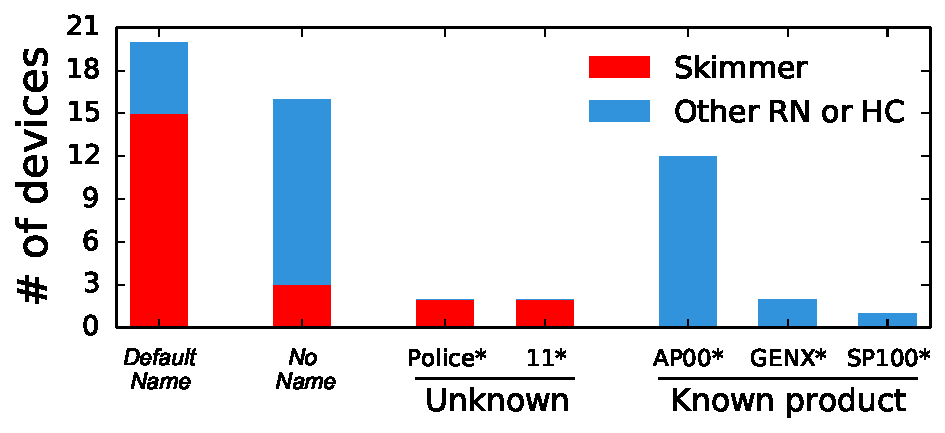
\includegraphics[width=\linewidth]{plots/bar_plot_name_cluster.pdf}
\caption{
  \label{fig:barplot_name_cluster}
  These modules are used in skimmers as well as other legit products commonly seen at gas stations. 
}
\end{figure}

Figure \ref{fig:barplot_name_cluster} shows a distribution of the Bluetooth names seen across gas stations for devices/products using either HC or RN module. We also show stacked bars to indicate how many of each category actually were recovered as skimmers. 
There are some interesting patterns here worthy of discussion:
\begin{prettylist}
	%
	\item \textbf{Legit products use these modules.} For instance, AP100* is a known name associated with On-Board Diagnostic readers that are found at smog check centres. SP100* and GENX* are the common product names of Bluetooth converter systems for car stereos. We verified these product names with our law enforcement contacts, and also by RSSI localizing these named products to smog check centres for AP00* and stores for audio devices.
	%
	\item \textbf{A large number of recovered skimmers use default name.} 75\% of modules with default RN or HC module name ended up being recovered as skimmers and therefore this in itself can be a reasonable marker for a skimmer. Note, however there are other kinds of module names that also can be skimmers, so we must be careful.
	%
	\item \textbf{Wierd names had sequential patterns.} We saw two "pairs" of module names at two different gas stations - \textit{(Police Survey 11, Police Survey 15)} and \textit{(110,111)}. While the names are random, they seem to be part of a sequence. Information from USSS tells us that these criminals are known to plant a number of these skimmers across multiple gas stations in a single \textit{skimming} run, and therefore the idea of sequential identifiers existing is possible. In fact in both the mentioned cases, all modules did turn out to be skimmers.
\end{prettylist}

This table lends credence to the idea that these commodity modules are very popular and are used in a variety of applications, including those that are common at gas stations. Therefore the mere presence of such a module at a gas station is not sufficient to warrant an inspection. Device names can be helpful in this regard but the question still remains : Is this sufficient or we need another piece of info?

\subsubsection{Where in the gas station are these modules?}

As described in previous sections, Bluetana enables localization of Bluetooth modules by real time RSSI updates. We mark all suspect modules (regardless of device name), so that data collectors can attempt to localize them to the vicinity of gas pumps. Figure shows Google Maps images of our localization attempt. Image on the left shows a skimmer module with default name close to the gas pumps, whereas image on the right is an AP00* device located in and around the smog check clinic.

Our survey has revealed to us the possible presence of a common skimmer modules at a certain number of gas station. In the next section, we validate our detection mechanism by calling in law enforcement
%}}}

\subsection{Evaluation: \bluetana is Accurate} %{{{

\paragraph{Recovering the skimmers}
Having performed the localization on site, we were able to confirm 15 skimmers across 6 gas stations in 2 different states which we reported to our law enforcement partners. They went in and thouroughly inspected all the gas pumps at all gas stations, and were able to recover the exact number of skimmers we reported. Our success rate therefore has been a 100\% so far.

While our methodology has been extremely successful in detecting skimmers (0\% false positive rate), we were faced with an important question. Because law enforcement only went in to inspect when we detected something, what if we were missing something? To answer this question we incorporated the help of Arizona States Weights and Measures department

\paragraph {Were there any false positives?}

To figure out how successful Bluetana was in a real world investigative scenario. we partnered with the state inspectors in Arizona Weights and Measures. As mentioned before state inspectors do regular complete inspections of gas stations based on routine or complaints. We deployed 3 phones with our app to 3 different inspectors, and they were willing to use our app and run scans whenever they went in for any form of inspection to a gas station. As Arizona state publicly releases reports of every single inspection performed, we were able to correlate our dataset of detected devices with individual inspection reports


\begin{table}[h]
\centering
\scriptsize
\resizebox{1\columnwidth}{!}{
\begin{tabular}{r|c|c|c}
%\cline{2-8}
%\multicolumn{1}{c|}{} & \multicolumn{8}{c|}{\cellcolor{black}\textcolor{white}{\textbf{\# of Gas Stations}} \\
% A & \textbf{None} & \textbf{ModuleA\n only} & \textbf{ModuleB\n only} & \textbf{Both} & T \\
\multicolumn{1}{c|}{} & \textbf{I$_1$} & \textbf{I$_2$} & \textbf{I$_3$} \\
\hline
\multicolumn{1}{r|}{\# of inspections}    &  6  &  13  &  8 \\
\rowcolor{lightgray}
\multicolumn{1}{r|}{Bluetana positive}   &  3  &  1  & 1   \\
\rowcolor{lightgray}
\multicolumn{1}{r|}{Skimmer recovered} & 1 & 1 & 0  \\
\multicolumn{1}{r|}{Bluetana negative}   &  3  &  12  & 7   \\
\multicolumn{1}{r|}{Skimmer recovered} & 1 & 1 & 0  \\
\hline
\end{tabular}
}
\caption{Distribution of inspections done by inspector(I$_n$). Table indicates low false positive and negative rates}
\label{tab:arizona_falsepositive}
\end{table}


* From the table we can see that the our false positive rate is fairly low. Only times when there was a false positive was in the case of transients, as in there was a vehicle/person at the location at that precise moment. More importantly there were only two cases of false negatives, and in those one of the cases the inspection for skimmers were done 11 days after the first time scanning was done using Bluetana. In the second case, the inspector drove past the gas station and was in the vicinity only for 6s which is not sufficient for even a single complete scan. Therefore we can conclude from real field analysis that even till date our false negative rate is very low or zero even.
%}}}

\subsection{Skimmers have similar MAC addresses} %{{{

\begin{figure}
\centering
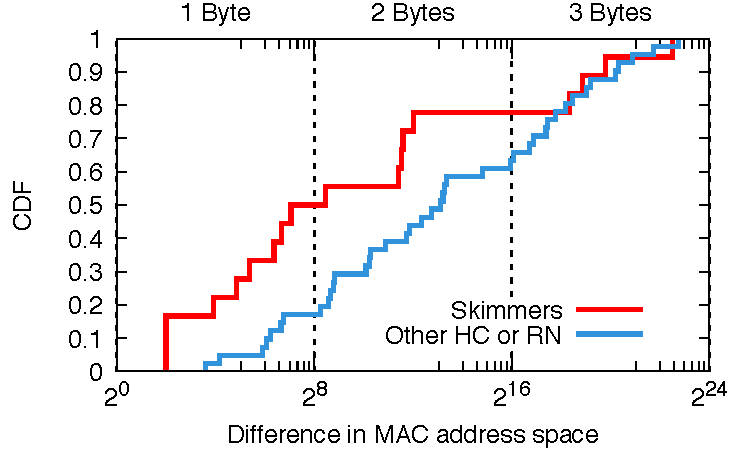
\includegraphics[width=\linewidth]{fig/hitlist_devices}
\caption{
\label{fig:hitlist_devices}
Skimmers are closer in MAC address space than other RN and HC-based Bluetooth devices.
}
\end{figure}

Next we looked to see if there is a pattern in the MAC addresses of skimmers
that we found indicating that the same criminals purchased the skimmers.
%
This investigation is inspired by prior work that found WiFi MAC address are
allocated by manufacturers sequentially during production~\cite{wifi-macs}.

To study this we computed the difference in MAC address space between a device
and the device that is next closest to it.
%
We did this for two separate set of MAC addresses: (a) those that were
confirmed to be skimmers, and (b) those that used the same Bluetooth modules,
but were not skimmers.

The distribution of the differences in MAC address space are shown in
Figure~\ref{fig:hitlist_devices}.
%
Skimmers are significantly closer in MAC address space to each other than other
devices:
%
half (11) of the skimmers we observed are within one byte (256 MAC addresses)
of another skimmer; whereas only 18\% of the of other RN and HC devices are in
the same distance.

We also discovered something very surprising,
%
Interestingly, this is similar to behavior that was discovered in
Nevada~\cite{ag-nevada-minutes}.
%}}}

\begin{table}
\centering
\scriptsize
\resizebox{1\columnwidth}{!}{
\begin{tabular}{r|c|c}
%\cline{2-8}
%\multicolumn{1}{c|}{} & \multicolumn{8}{c|}{\cellcolor{black}\textcolor{white}{\textbf{\# of Gas Stations}}} \\
% A & \textbf{None} & \textbf{ModuleA\n only} & \textbf{ModuleB\n only} & \textbf{Both} & T \\
\textbf{City} & \textbf{Skimmers recovered} & \textbf{Population} \\
\hline
A  & 12 & 1,339,000  \\  
B   & 4 & 185,038     \\
C 	&  2  & 501,344 \\
D & 2 & 40,224 \\
E & 2 & 36,064 \\
F & 1 & 4,737,270 \\
G & 1 & 151,969 \\
\hline
\end{tabular}
}
\caption{Distribution of skimmers recovered by Bluetana by metropolitan area. Names of cities are not revealed but their populations have been mentioned.}
\label{tab:skimmer_chest}
\end{table}
\end{comment}
\begin{comment} % extra text {{{



\subsection {Are we missing anything?}

As seen previously, we have had a 100\% success rate in detecting skimmers across multiple regions in the US. Since law enforcement officials were opening up pumps only when reported the gas stations to them, we needed to perform a different study to figure out the robustness of our methodology. The biggest question being : when implemented in a real world scenario, what is the false positive and false negative rate of Bluetana?

To answer this question we partnered with the state inspectors in Arizona Weights and Measures. As mentioned before state inspectors do regular complete inspections of gas stations based on routine or complaints. We deployed 3 phones with our app to 3 different inspectors, and they were willing to use our app and run scans whenever they went in for any form of inspection to a gas station. As Arizona state publicly releases reports of every single inspection done, we were able to correlate our dataset of detected devices with individual inspection reports

Table below summarises the results of using Bluetana in 

* Table of Arizona number of inspections per inspector (if possible), number of gas stations where Bluetana was used on or a previous inspection date, Bluetana positive no of gas stations, bluetana negative no of gas stations, if positive number of devices revealed, number of inspection where they found skimmers 

* From the table we can see that the our false positive rate is fairly low. Only times when there was a false positive was in the case of transients, as in there was a vehicle/person at the location at that precise moment. More importantly there were only two cases of false negatives, and in those one of the cases the inspection for skimmers were done 11 days after the first time scanning was done using Bluetana. In the second case, the inspector drove past the gas station and was in the vicinity only for 6s which is not sufficient for even a single complete scan. Therefore we can conclude from real field analysis that even till date our false negative rate is very low or zero even.
%\end{comment}
\begin{comment}

\subsubsection{What about Module B?}

We address the case of Module B separately because of some interesting insights. During our initial drives, we observed hardly any Module B activity across any gas stations, making us wonder if we were missing something. To address this, we ran an experiment where we bought samples of Module B sourced from multiple different online portals, with the aim of identifying if there was a difference.

An interesting observation was that while the boards had the same exact PCB design, including Bluetooth radio chipset manufacturer, the MAC address they advertized with was in a variety of address space ranges.

\begin{table}[h]
\centering
\resizebox{1\columnwidth}{!}{
\begin{tabular}{rc}
%\cline{2-8}
%\multicolumn{1}{c|}{} & \multicolumn{8}{c|}{\cellcolor{black}\textcolor{white}{\textbf{\# of Gas Stations \\
 A & \textbf{None} & \textbf{ModuleA\n only} & \textbf{ModuleB\n only} & \textbf{Both} & T \\
\hline
\textbf{Module Source} & \textbf{MAC address range} \\
\hline
Source 1 & 20:18:XX:XX:XX:XX \\
Source 2 & 98:D3:32:XX:XX:XX \\
Source 3 & 20:17:XX:XX:XX:XX \\
\hline
\end{tabular}
}


\caption{Different MAC ranges observed for Module B purchased from different sources}
\label{tab:ModuleB_MAC}
\end{table}
What is interesting about these address ranges is that these follow IEEE guidelines for OUI ranges (2nd lowest bit of MSB is unset), which implies these are a globally unique addresses. However these address ranges are listed neither in the public nor the private listing of IEEE Address ranges, almost as if the modules are MAC squatting. 

Taking this as an insight into how Module B manufacturers choose MAC addresses, we modified our tool to indicate such devices in red as well. Also we went back to our already collected database, and saw that in the past we had seen about 13 such modules over past several months. We observed that all of these modules either had the default trade name or no name at all, which meant no further filtering was possibleWith a long time having passed between the last sighting, our expectations of catching the modules were not high. Despite this we proceded to perform a confirmation at all the gas stations where the modules were seen. 

While in most cases we werent able to see the module again, in two gas stations in two different states we were able to detect presence and localize to gas pumps a total of 3 Module Bs. Our law enforcement partners were able to recover all the modules we reported in both the gas stations. What was quite interesting and scary, to think about it was that these particular modules were recovered almost 3 and 4 months after they were first detected by one of our data collectors. This in a way lends credence to our argument about how these modules can stay for a long time in gas dispensers continuously skimming card information.
As discussed previously, one of the major challenges with Bluetooth skimmer is that they are short range. Therefore detection and can only be achieved by driving to gas stations itself. For validation of our methodology, we decided to do a large scale survey by driving to gas stations in our county

\subsection {Setup of the experiment}

Table \ref{tab:countystats} shows the statistics of population and gas stations in our county. With such a large number of gas stations, a complete survey with a small number of researchers was difficult in a reasonable amount of time. We needed to cut down our search space based on a reasonable heuristic.

\begin{center}
\begin{tabu} to 0.8\columnwidth { | X[l] | X[c] | }
 \hline
 \textbf{Geographic Area} & 4526 sq mi \\
 \hline
 \textbf{Number of cities}  & 18 \\
 \hline
 \textbf{Population density} & 680/sq mi \\
 \hline
 \textbf{Number of gasoline stations} & 873 \\
\hline
\end{tabu}
\label{tab:countystats} 
\end{center}

As has been discussed previously, gas dispensers suffer from a variety of vulnerabilities because of which the CRIND tray is easily accesible. One particular kind, are a three upper door style dispensers, of which one of the doors provides access to the CRIND internals (Figure \ref{fig:gilbarcoadvantage}). This upper door has a key access to open, and the key as discussed previously can be purchased online. We confirmed with our law enforcement sources, that these particular ones are some of the commonly targeted. 

\begin{figure}
\centering
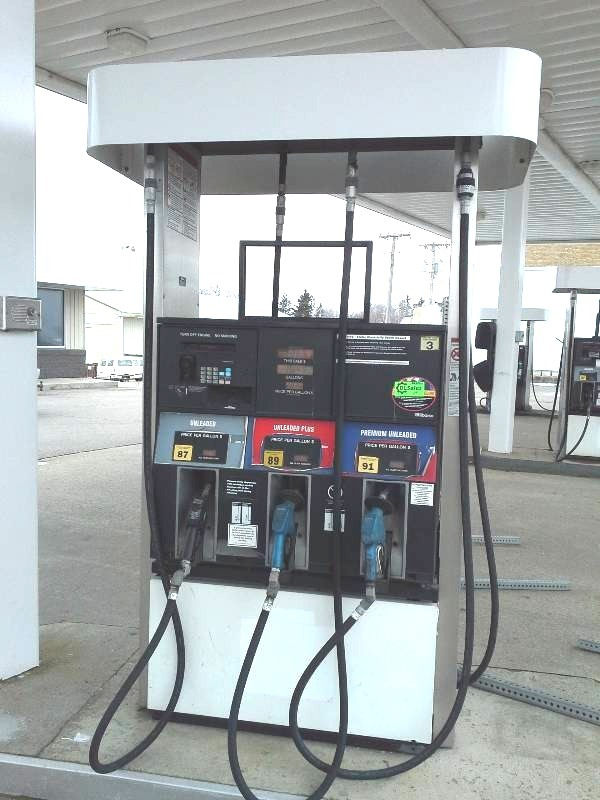
\includegraphics[height = 8cm,width = \columnwidth]{fig/gilbarcoadvantage.jpg}
\caption{Gas stations using these 3 door style dispensers were the focus of our validation effort. The upper left door has the CRIND tray accesible via a key slot}
\label{fig:gilbarcoadvantage}
\end{figure}

We obtained gas station coordinates of all gas stations from the county's public GIS database. Using these coordinates, we were able to run Google Street view search for each of the 873 gas stations. We can view individual gas dispensers at gas stations by zooming into the street view images (Figure . By manually inspecting the images, we identified 208 gas stations in the county, that use this particular type of gas dispenser.

\begin{figure}
\centering
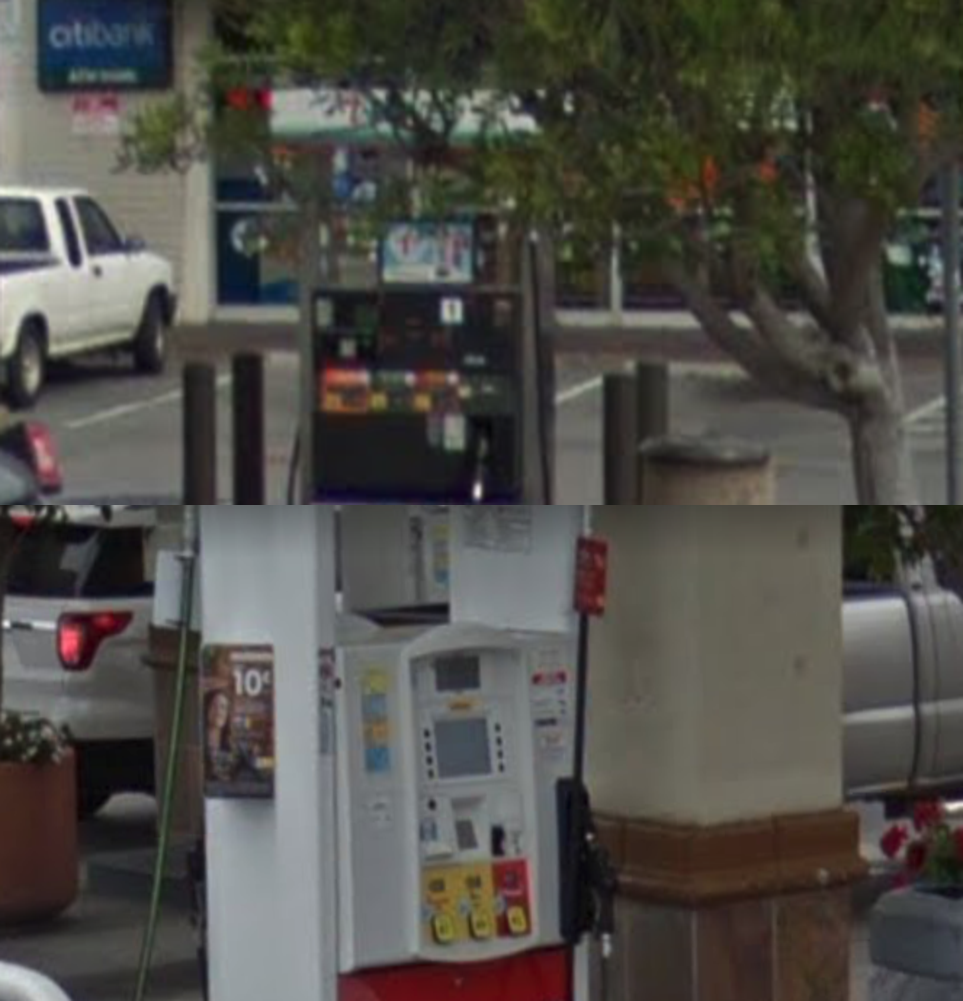
\includegraphics[height = 8cm,width = \columnwidth]{fig/googlestreet.pdf}
\caption{Google street view images for identifying gas dispenser type at a gas station. Photo on top is the gas dispenser we are targeting, whereas image on bottom is a different kind}
\label{fig:googlestreet}
\end{figure}

With the number of gas station down to a reasonable number, we drove to all gas stations to inspect for presence of skimmers and validate our methodology. We discuss the results in the next section.

\subsection{Results}

\begin{figure}
\centering
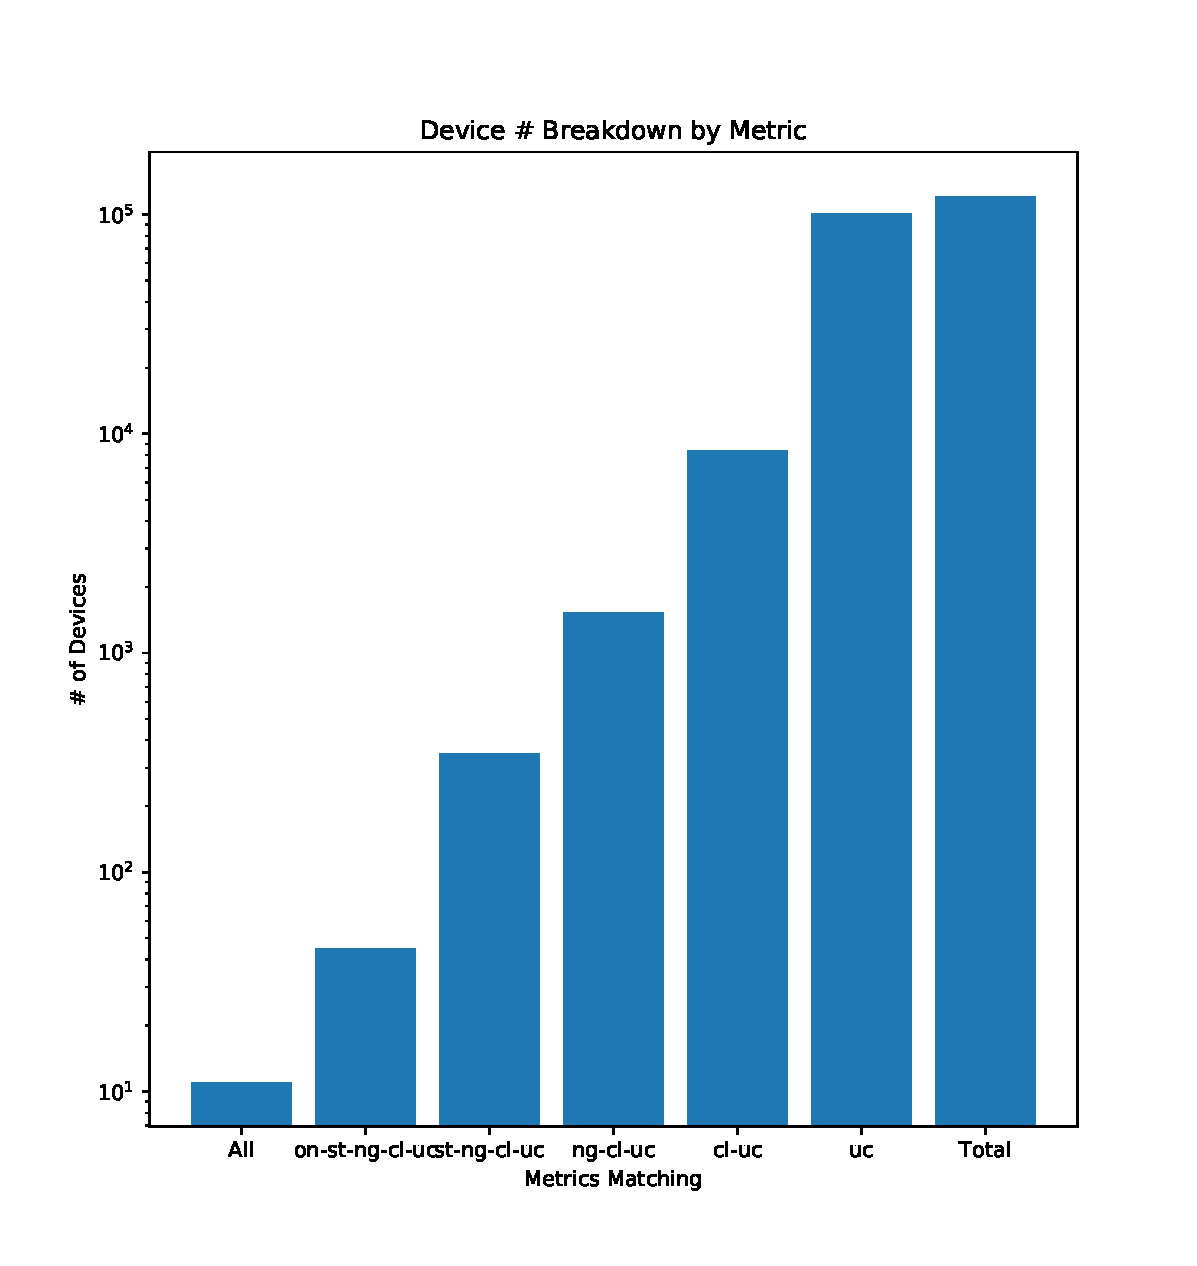
\includegraphics[width=\linewidth]{fig/dbstats}
\caption{
\label{fig:dbstats}
Bluetooth wardriving dataset overview \todo{Update with latest numbers}.
}
\end{figure}

Having implemented both a scalable mechanism for skimmer detection as well as
having ``deployed'' the mechanism at a large scale to measure hundreds of gas
pumps, we collected data on both the general bluetooth environment as seen from
a person driving in a car down the highway and the specific bluetooth environments
of locations such as gas stations, coffee shops, parks, and downtown areas.

In total, we recieved 2,217,611 enquery response packets with data of discovered
devices, and 137,620 unique IEEE MAC addresses. Of these two million responses,
251,795 were within a half mile of a gas station, and amongst these responses are
22,344 unique MAC addresses. \todo{From this, say how many matched the hitlist,
how many are not on the whitelist.} \todo{More device breakdown?}

- Here's what we saw from our crowdsourced data collection
- How many gas stations you have been to.
- Pick out bad manufacturers
- It is still a lot of stuff, so we generate a whitelist for a device

- Detection Methodology

- We need to validate our opinions so we do a study
- Here's what we saw from the survey of the gas station data
- We found these skimmers
- Here's a case where we found a skimmer
- Here's a case where we did not find a skimmer


We gathered inquiry responses from many gas stations in California, and created
simple filters for these fields to find devices that match the profile of one
of the wireless modules that can be used as a skimmer, and has been
seen before to be involved in skimmers (see our strategy for crowdsourced data
gathering for implant detection described in Section~\ref{sec:crowdsourcing}). 

Figure~\ref{fig:dbstats} shows an overview of the Bluetooth devices that we
observed.
%
\todo{Each field reduces the number of suspected implants by an order of
magnitude.}
%
This indicates that each field can be very useful in reducing the number of
potential implants. 
%
Figure~\ref{fig:dbstats} shows the results of this initial drive. Preliminary
Bluetooth scans around gas stations in California revealed 30,420 unique
Bluetooth MAC addresses, of which our preliminary Bluetooth-specific detection
techniques brought down to 70 likely targets, of which 4 were confirmed gas
station skimmers that were eventually recovered by the US Secret Service.
\end{comment} 
%}}}
